%%%%               %%%%
%%%% PLANIFICACIÓN %%%%
%%%%              %%%%

\chapter{Planificación}
\label{chap:planificación}

\lettrine{L}{a} creación de este TFG comparte las características generales de cualquier proyecto, ya que tiene un objetivo concreto y definido, no es una actividad rutinaria, tiene unas fechas de comienzo y de fin. Un proyecto necesita recursos en forma de tiempo, mano de obra, herramientas y conocimiento. En este capítulo se aborda la planificación elaborada.

\section{Recursos necesarios}

Para acometer el proyecto son necesarios varios tipos de recursos:

\begin{itemize}
    \item \textbf{Humanos}
        \begin{itemize}
            \item Un Product Owner, rol asignado al director del proyecto.
            \item Un analista.
            \item Un diseñador.
            \item Un equipo de desarrollo, formado íntegramente por el alumno.
        \end{itemize}
    \item \textbf{Software}: todos los recursos software utilizados son aplicaciones sin coste económico, mucho de ellos, además, software libre.
    \item \textbf{Hardware}: el portátil, pantalla y otros accesorios utilizados.
\end{itemize}

El rol de Product Owner lo realiza el director del proyecto, como se explicó en la Sección \ref{sec:uso-scrum-en-el-proyecto}. Las funciones de análisis, diseño y desarrollo fueron asumidas por el alumno. Cabe destacar que la colaboración para la creación de una interfaz gráfica a este proyecto fue realizada por otro alumno de la Facultad de Informática, no obstante debe quedar claro que no intervino en ningún momento en la elaboración de la parte del trabajo presentada en esta memoria.

\subsection{Planificación económica}

De los recursos utilizados para el proyecto se deducen directamente los costes económicos incurridos. En la Tabla \ref{tab:costes-proyecto} se presentan todos los gastos. Para el cálculo de los costes salariales se consultó el \emph{Convenio colectivo del sector de empresas de ingeniería y oficinas de estudios técnicos} en su página del BOE \footnote{\url{https://www.boe.es/diario_boe/txt.php?id=BOE-A-2019-14977}}.

\begin{table}[ht]
    \centering
    \begin{tabular}{l l l l}
        Recurso & Coste (€/h) & Tiempo (h) & Coste total (€) \\
        \hline
        \hline
        Jefe de proyecto & 42 & 18 & 756 \\
        Analista & 35 & 65 & 2275 \\
        Diseñador & 35 & 50 & 1750 \\
        Programador & 30 & 445 & 13350 \\
        Equipamiento informático & -- & -- & 900 \\
        Microsoft Project (licencia universitaria) & -- & - & 0 \\
		Otro software & -- & - & 0 \\    
        \hline
        \hline
        TOTAL & & - & 19031 \\        
    \end{tabular}
	\caption{Costes del proyecto}    
	\label{tab:costes-proyecto}
\end{table}

\section{Planificación temporal inicial}

En la Imagen \ref{fig:gantt-inicial} se presenta el diagrama de Gantt inicial de la planificación con el desglose de tareas. Una de las dificultades para la planificación consistió en no saber en qué momento del proyecto sería necesario abordar la integración con la interfaz web. Inicialmente se asumió que ocurriría durante el trabajo de desarrollo y antes de comenzar la escritura de la memoria. En este plan inicial se contemplan 520 horas de trabajo.

\begin{figure}[hp!]
    \centering
    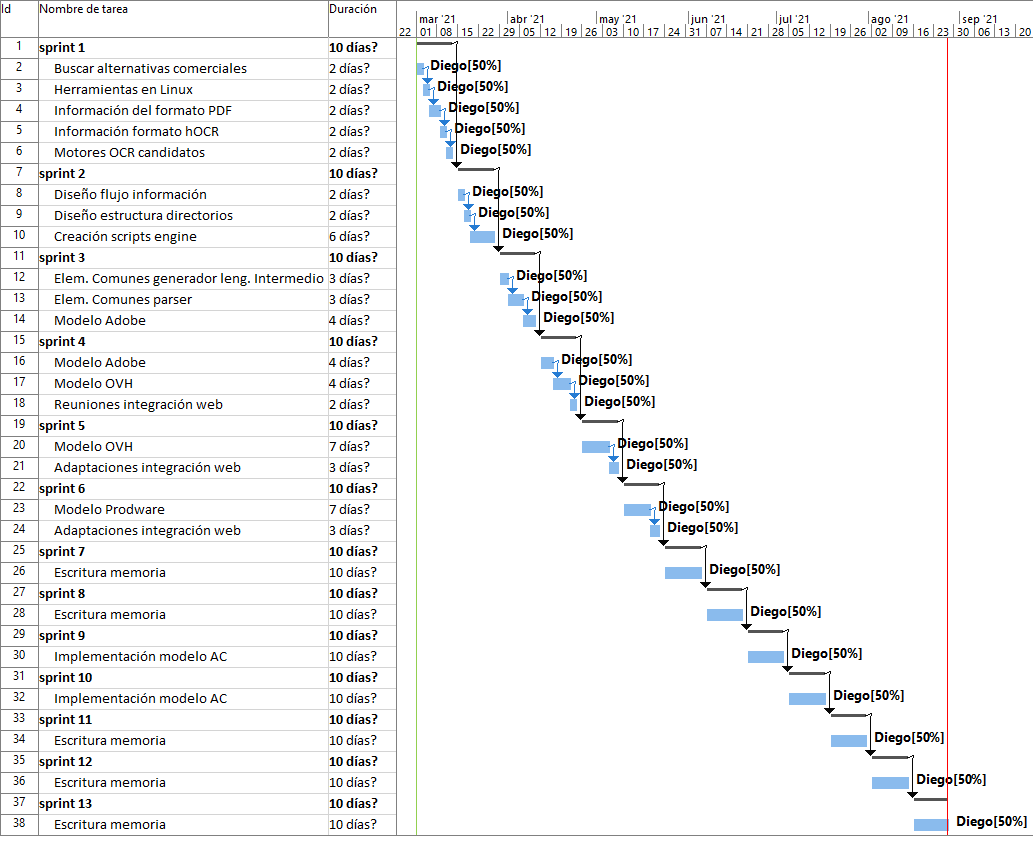
\includegraphics[angle=90,width=1.0\textwidth]{imaxes/f-planificacion/gantt-inicial.png}
    \caption{Diagrama de Gantt y tareas iniciales del proyecto}
    \label{fig:gantt-inicial}
\end{figure}

\section{Sprints}

Se expone a ahora la distribución del trabajo a lo largo de los Sprints. Por motivos de compatibilidad a nivel laboral y otras responsabilidades personales, se optó por una fórmula de 20 horas de trabajo semanal y Sprints de 5 días (de lunes a viernes). Al realizarse a media jornada, los Sprints tiene dos semanas reales de duración, completando de esta manera una jornada completa en cada uno.

\subsection{Sprint 1}

Este primer Sprint consiste por completo en un Spike con el objetivo de recabar toda la información necesaria para plantear el proyecto a nivel técnico. Algunos de los aspectos sobre los que se necesita adquirir conocimiento son:

\begin{itemize}
    \item Alternativas comerciales en la misma temática.
    \item Herramientas y librerías disponibles en Linux para manipular PDF.
    \item Funcionamiento del formato PDF a nivel interno.
    \item Formatos de salida de los motores de OCR, en especial del seleccionado, hOCR.
    \item Posibles \emph{engines} de OCR candidatos para el proyecto
\end{itemize}

\subsection{Sprint 2}

Con el conocimiento adquirido se procederá a la construcción inicial del sistema para el procesamiento por lotes de los trabajos. Además de diseñar la estructura de directorios utilizada por el proyecto, se crearán el Makefile general, utilizado para las compilaciones y los \emph{scripts} para implementar el motor.

\subsection{Sprint 3}

En el Sprint 3 crearán las implementaciones iniciales del generador de lenguaje intermedio y se preparará el primer \emph{parser}, que se probará con los documentos de Adobe. Para la construcción de los analizadores léxico-sintácticos se desea un enfoque modular, que no es la fórmula directa con este tipo de herramientas. Construir la herramienta siguiendo esta aproximación llevará más tiempo que el habitual en el caso de escoger un planteamiento más sencillo.

\subsection{Sprint 4}

En el Sprint 4 se añadirá soporte para la generación de código intermedio y \emph{parsing} del modelo de Adobe y parte del de OVH. Se reservarán algunas horas del Sprint para las reuniones de cara a prepara el prototipo web y cuales adaptaciones serán necesarias.

\subsection{Sprint 5}

Se completará el modelo de documento del proveedor OVH. Además se abordarán de forma paralela las tareas relacionadas con el prototipo web. También en este Sprint se reservarán horas para las reuniones que sean necesarias con motivo del prototipo web. Con seguridad se necesitará tiempo para discutir cualquier aspecto técnico no considerado inicialmente.

\subsection{Sprint 6}

El Sprint 6 se dedicará a realizar el modelo de Prodware y a finalizar la integración con la aplicación web.

\subsection{Sprints 7 y 8}

En estos dos Sprints se abordará la escritura inicial de la memoria, con la previsión de dejar tiempo al final del proyecto para completarla.

\subsection{Sprint 9}

Implementación del modelo de AC, basado en imagen.

\subsection{Sprint 10}

Implementación del modelo de AC, basado en imagen.

\subsection{Sprints 11 al 13}

Los últimos Sprints se dedicarán a completar la escritura de la memoria.

\section{Análisis de riesgos}

En esta sección se identifican de forma priorizada riesgos que podrían impedir, o al menos dificultar, completar el proyecto según lo previsto. Se comentan acciones de mitigación en cada caso:

\begin{itemize}
	\item \textbf{No encontrar ninguna herramienta capaz de extraer las coordenadas} de los elementos de un documento. Si no se dispusiese de los datos para poder emparejar las plantillas tampoco se podría avanzar con el proyecto tal como se plantea inicialmente. En ese caso se podría replantear el proyecto para incluir la generación de coordenadas y descartar otras funcionalidades.
	
	\item \textbf{Algún aspecto del desarrollo, o de la elaboración de la memoria, podría llevar más tiempo del considerado.} Se debe reservar un margen temporal suficiente al final del proyecto para asumir desvíos, en lugar de planificar las tareas del proyecto hasta la fecha máxima de entrega.
	
	\item \textbf{Cambios de alcance en la integración con la interfaz web} para incorporar funcionalidades que excedan el tiempo reservado. En este caso se intentaría negociar el número de \emph{features} y se propondría dividir el trabajo en partes, intentando dejar para el futuro las características que menos valor aporten.
	
	\item \textbf{Destrucción o robo de la máquina de desarrollo} en algún momento del proyecto. Todo el trabajo realizado debe ser replicado a repositorios remotos, como Github. En el caso de ficheros que no necesiten versionado, se deberá realizar copias periódicas en el almacenamiento en la nube proporcionado por la universidad. Actualmente se dispone de otros ordenadores que podrían ser utilizados una vez se instale el entorno.

	\item \textbf{Enfermedad del alumno}, y desarrollador principal, que impida avanzar el proyecto. Al ser un trabajo de carácter personal, no transferible a otra persona, no habría acción posible y supondría la cancelación si se consume todo el tiempo disponible.

	\item La \textbf{disponibilidad de horaria} para completar el trabajo está ligada al disfrute de una jornada laboral de 7 horas durante el verano. En caso no disfrutar de esta reducción horaria se podría pedir una excedencia para poder completar el trabajo en tiempo, o utilizar las vacaciones.

	\item \textbf{Selección de alguna tecnología que cese de tener soporte en forma de un equipo de desarrollo que realice mantenimiento y mejoras.} Probablemente la tecnología más frágil en este sentido sea la formada por Flex y Bison. Especialmente el primero solo tienen un mantenedor en la actualidad. Deberían considerarse algunos de los analizadores alternativos como ANTLR \footnote{\url{https://www.antlr.org/}}. Este riesgo afectaría al proyecto no inmediatamente sino a largo plazo.


\end{itemize}

\section{Planificación temporal final}

La planificación final tuvo un desvío claro en la elaboración de la memoria, que finalmente llevó cuatro semanas más de las previstas (2 Sprints), haciendo un total de 560 horas. Así mismo, para ir incorporando los sucesivos documentos fue necesario cierto retrabajo en la parte del generador de código intermedio, al tener que ampliar sus funcionalidades, manteniendo los resultados conseguidos hasta el momento. Las reuniones de integración sucedieron, aproximadamente, dentro del periodo esperado, antes de dar comienzo a la primera parte de la escritura de la memoria. El resultado final de la planificación se puede consultar en la Imagen \ref{fig:gantt-final}.

\begin{figure}[hp!]
	\centering
	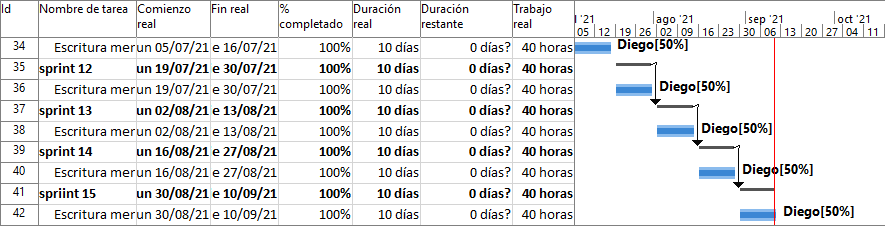
\includegraphics[angle=0,width=1.0\textwidth]{imaxes/f-planificacion/gantt-final}
	\caption{Diagrama de Gantt del final del proyecto}
	\label{fig:gantt-final}
\end{figure}
